\documentclass[11pt,a4paper,oneside]{article}

\usepackage[utf8]{vietnam}
\usepackage[english]{babel}
\usepackage{freecontest}
\usepackage{verbatim}
\usepackage{graphicx}
\usepackage{wrapfig}

\header{\LARGE Free Contest 118}

\begin{document}

\problemtitle{ANHSANG}
\\
Một trong những vấn đề kinh điển trong đồ họa máy tính là bài toán xác định độ sáng của một điểm bất kì trong không gian. Hôm nay, các bạn thí sinh Free Contest sẽ có cơ hội giải một phiên bản được đơn giản hóa của bài toán này. \\\\
Cho một căn phòng có dạng một hình đa giác không tự cắt trên mặt phẳng $Oxy$ và một điểm sáng nằm hoàn toàn trong đa giác này. Điểm sáng này sẽ toả ra xung quanh nó những tia sáng thẳng, những tia sáng này chỉ có thể bị chặn lại bởi những bức tường là các cạnh của đa giác. Hãy viết chương trình tính phần diện tích được chiếu sáng.
\heading{Dữ liệu}
\begin{itemize}
\item Dòng đầu tiên gồm hai số thực $x_0, y_0$ là vị trí của điểm sáng.
\item Dòng thứ hai gồm một số nguyên dương $n$ ($3 \leq n \leq 10000$) là số đỉnh của căn phòng hình đa giác.
\item $n$ dòng tiếp theo, dòng thứ $i$ gồm hai số thực $x_i, y_i$ là tọa độ của một đỉnh của đa giác. Các đỉnh được cho theo thứ tự ngược chiều kim đồng hồ.
\end{itemize}
Các số thực trong dữ liệu vào sẽ có giá trị tuyệt đối không vượt quá $1000$ và có không quá bốn chữ số sau dấu phẩy thập phân. Ngoài ra, không có hai đỉnh nào của đa giác trùng nhau và không có bộ ba đỉnh liên tiếp nào của đa giác thẳng hàng (lưu ý rằng ba đỉnh không liên tiếp của đa giác vẫn có thể thẳng hàng với nhau).
\heading{Kết quả}
\begin{itemize}
\item Gồm một số thực làm tròn đến đúng hai chữ số sau dấu phẩy thập phân là diện tích phần được chiếu sáng của căn phòng.
\end{itemize}
\heading{Ví dụ}
\begin{example}
\exmp{%
813.9707 765.1039
8
774.4324 496.7201
939.6262 867.0015
727.8536 931.5901
339.6567 678.8505
-82.0790 856.0738
-583.7845 981.4783
-574.0556 -478.5426
446.0628 -228.9920\\
}{%
1254952.38
}%
\end{example}
\newpage
\heading{Giải thích}
\begin{center}
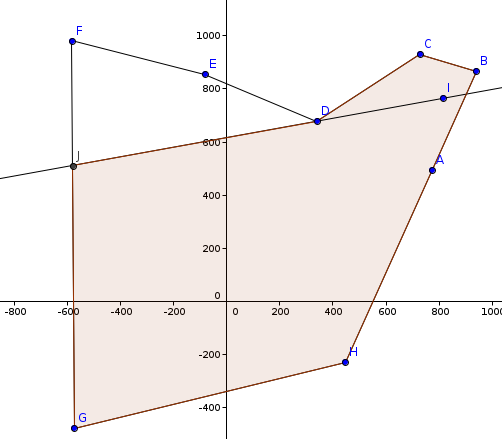
\includegraphics[scale=1.0]{anhsang.png}
\end{center}
Căn phòng trong ví dụ có dạng hình đa giác $ABCDEFGH$ và điểm sáng $I$ nằm hoàn toàn trong căn phòng. Điểm sáng này chiếu sáng đa giác $ABCDJGH$ có diện tích 1254952.38
\heading{Chấm điểm}
\begin{itemize}
\item Trong 20\% số test tương ứng với 10 điểm, căn phòng được cho có dạng một hình đa giác lồi.
\item Trong 80\% số test còn lại tương ứng với 40 điểm, căn phòng được cho có dạng một hình đa giác lõm. 
\end{itemize}
\end{document}